\documentclass[letter,11pt]{article}
%\documentclass[letter,10pt]{scrartcl}

\usepackage[utf8]{inputenc}
\usepackage[pass,letterpaper]{geometry}
\usepackage{graphicx}
\usepackage{listings}
\usepackage{color}
\usepackage{float}
\usepackage{bigfoot}
\usepackage[square,sort,comma,numbers]{natbib}
\usepackage{titling}
\usepackage{mathtools}
\usepackage{helvet}
\usepackage{algorithmicx}
\usepackage{algpseudocode}

\setlength{\parindent}{0cm}

\title{OpenMemDB: A wait-free database\thanks{Sponsor: Dr. Damian Dechev}}
\author{Michael McGee \and Robert Medina \and Neil Moore \and Jason Stavrinaky}
\date{2/1/2016}

\pdfinfo{%
  /Title    (OpenMemDB: A wait-free database)
  /Author   (Mike McGee, Neil Moore, Robert Medina, Jason Stavrinaky)
  /Creator  ()
  /Producer ()
  /Subject  ()
  /Keywords ()
}

\let\oldReturn\Return
\renewcommand{\Return}{\State\oldReturn}

\definecolor{codegreen}{rgb}{0,0.6,0}
\definecolor{codered}{rgb}{0.6,0,0}
\definecolor{codegrey}{gray}{0.9}

\newcommand{\inlinecode}[1]{\colorbox{codegrey}{\lstinline[language=C++]{#1}}}

\begin{document}
\pagenumbering{gobble}
\maketitle
\newpage

\pagenumbering{arabic}

\section{Introduction}
While hard drives are getting faster, they are still relatively slow when compared 
with main memory while memory is getting cheaper. Memory is following a long running 
pattern where it has precipitiously dropped from costing thousands of dollars for a few 
megabytes to about \$40 for 8 gigabytes \cite{jcmit}. With this trend, we can take 
advantage and design extremely fast databases. While there are many applications for 
which current database solutions are fast enough (website logins for example), these 
solutions leave something to be desired for massively concurrent systems with high throughput
requirements such as real-time analytics on large datasets. While the largest of 
these datasets are still too large for main memory, some datasets are finally able
to fit into main memory in modern systems due to the cheapness and advancement of 
memory module technology. Making it possible for a data analysis algorithm to make 
full use of the database server's processing power to extract and manipulate data
would make that analysis quicker and efficient in terms of hardware use.
\par\vspace{\baselineskip}
A real-world example of this need for fast and high throughput databases is demonstrated by Zynga, 
the developers of Words with Friends and Farmville, faced a problem where their 
database was not able to supply their data analysis algorithm problem. With so 
many users, their database solution was not fast enough to provide real time analytics. 
There were just too many transactions going on at once. They 
remedied this by switching to MemSQL: a closed-source in-memory database. With this 
solution, Zynga can ``make decisions based on billions of data points in real-time to 
provide better in-game personalization and overall customer satisfaction''. \cite{MemSQL} 

\subsection{Motivation}
Over the last 30 years the there has been tremendous advancements in computing
hardware. "Processors are thousands of times faster and memory is thousands of
times times larger"\cite{stonebraker2007end}. Most technologies have advanced 
along with hardware, however database management systems have struggled to improve
at a similar rate. This is mostly due to concurrency issues. "Existing studies show
that current database engines can spend more than 30\% of time in 
synchronization-related operations (e.g.locking and latching), even when only a 
single client thread is running."\cite{soares2015database}
\par\vspace{\baselineskip}
OpenMemDB attempts to solve this problem by implementing a data-store using only wait-free data
structures. This leads to performance that scales with increasing threads. OpenMemDB also
resides completely in-memory and therefore avoids all of the slow downs associated with
going to disk.
\par\vspace{\baselineskip}

\section{Related Work}
There have been some attempts to increase the performance of database management
systems in recent years. Some solutions will sacrifice
some data consistency in order to achieve better performance. Still others
remain fully ACID compliant and attempt to parallelize individual steps in the 
DBMS or solely use multiple threads when executing query plans. Then there are those
that attempt to implement some level of lock freedom into their DBMS.
\par\vspace{\baselineskip}
\subsection{MemSQL and VoltDB}
MemSQL\footnote{MemSQL can be configured as a Columnstore that stores data on disk}
and VoltDB are both fully in-memory DBMS as is OpenMemDB. This is where the
similarities end as far as OpenMemDB is concerned. MemSQL and VoltDB on the other 
hand both use distributed systems to achieve performance gains. MemSQL differs from 
VoltDB in a few ways, the most important being its use of lock-free data structures
for storing data and its storing of pre-compiled commonly used queries\cite{MemSQL}.
VoltDB tries to make its performance gains by what they call "Concurreny through
scheduling."\cite{VoltDB} This is the process of using a single-threaded pipeline 
that performs the task it was scheduled. This limits the need for locking during
transactions by intelligently scheduling the transactions so that locks are not
necessary.
\par\vspace{\baselineskip}
OpenMemDB aims to take a different approach, one that is fully wait-free. The goal is 
to use powerful wait free data structures that will allow for a massively parallel 
DBMS that can scale with the addition of processors and memory. It is our assumption 
that the achievement of a fully weight free DBMS will achieve the performance gains 
that have been lacking in the DBMS world while eliminating the complexity of 
distributed systems, all while retaining full ACID compliance.
\newpage

\section{Technical Approach}
Our database is built upon wait-free data structures found in Tervel, a collection of
lock-free and wait-free data structures created by Dr. Damian Dechev et al\cite{web:tervel}. We use
the common definition of wait-freedom as found in Herlihy's definitive text\cite{herlihy:waitfree}, which
also provides us with the proof that the composition of linearizable algorithms or data structures
is also linearizable. From the beginning we knew that in order to create a
composition of linearizable parts and thus be able to prove linearizability, which is a core component of
wait-freedom, communication between the various threads must be minimized and only
done through the wait-free data structures and algorithms available to us. From there
we can then prove that all running threads are guaranteed to make progress in some finite time
and then prove wait-freedom from that foundation.
\par\vspace{\baselineskip}
The architecture of our database is fairly straightforward, with three main modules that 
communicate with each other: the Work Manager, SQL Engine, and Data Store. The communication
between modules is facilitated by a template function that each worker thread, in isolation, uses.
Each module has a distinct responsibility and mechanism of fulfilling that responsibility with as 
little communication between threads as possible. The Work Manager is responsible for distributing
incoming queries and commands among the worker threads as well as sending the final results of those
queries or commands back to the client that sent them. The SQL Engine is responsible for parsing the
given query or commmand string into an internal representation that can be executed on the Data Store.
The Data Store is where all the database's data is stored and thus is where the wait-free data
structures are mainly used. Those wait-free data structures are important to guarantee that all
the worker threads can safely and efficiently execute their assigned tasks and then communicate
those results to the Work Manager.
\par\vspace{\baselineskip}
Each worker thread is a long-lived thread spawned by the database upon startup and has various
thread-local pieces of memory given to it that are used by the various modules. Each instance of
this memory is guaranteed to be only be accessible by the assigned thread by the C++11 standard\cite{std:c++11}.
Most of this memory is used by the parser engine within the SQL Engine module and when the 
thread enters that module, there is zero shared state between it and another thread. When the thread
leaves the SQL Engine and proceeds to execute the parsed statement, it calls the appropriate
method within the Data Store module. This begins the portion of the database where the data 
structures and algorithms are heavily relied upon to achieve linearizability and wait-freedom.
We specifically use a wait-free hash-map to relate table names to the tables themselves which are nested
wait-free vectors. The composition of the Tervel vectors to create the table structure is such that the outer
vector acts as a container of references to records within the table while each of the referenced vectors
contain the stored data. Access to these data structures is minimized to reduce code complexity and 
possible contention between threads over the data contained in the structures.
\par\vspace{\baselineskip}
Specifically, the Data Store methods used by the worker threads make local copies of the data contained
in the core data structures as much as possible so as to take advantage of the standard library's
well-defined and optimized containers. This also allows us to concretely define the situations where 
multiple writers attempt to write to the same element in the shared data structures. In the few situations
this can occur, namely in the event of multiple concurrent SQL UPDATE or DELETE statements, we only perform
the operation if the targeted record hasn't been changed. This is done using Tervel's compare-and-swap 
operation on a particular element in the vector. Failing to perform these operations due to the 
selected record(s) changing between the time of selection and the time to perform the operation
is deemed a soft failure due to contention between threads executing concurrent and overlapping statements
and is communicated to the client as such.
\par\vspace{\baselineskip}
Inserting records into a table within the Data Store requires pre-processed data be passed
into the insertRecord method of the Data Store object. The general proecedure of inserting
into a table is shown in Figure \ref{insert_record}. This method first retrieves the table 
that we want to insert into and ensures the data provided adheres to the schema defined 
at the table's creation. Assuming that check is successful, a Tervel vector is then 
constructed using the given data while preserving the order of the data. Once the vector 
is setup we then push the final vector into the table.

\begin{figure}
 \begin{algorithmic}
 \Function{InsertRecord}{TableName, Data}
 \State{T = \Call{GetTable}{TableName}}
 \If{$\Call{SchemaCheck}{$T, D$}\neq True$}
  \Return{$False$}
 \EndIf
 \State{R is a Tervel vector}
 \ForAll{D in Data}
  \State\Call{PushBack}{R,D}
 \EndFor
 \State\Call{PushBack}{T,R}
 \Return{$True$}
 \EndFunction
 \end{algorithmic}
 \caption{How a record is inserted into a table in OpenMemDB}
 \label{insert_record}
\end{figure}

\par\vspace{\baselineskip}
Our handling of read-only operations is similar to the relativistic programming approach detailed 
in Howard and Walpole's paper on relativistic red-black trees, where each reader of the 
data structures only works within its own temporal frame of the data structure\cite{rbtree}. 
This is done by copying to local unshared memory and then manipulating the data, 
effectively capturing a snapshot of the data that we then use to generate the final 
output given to the client. This manipulation of the data is bounded and cannot 
infinitely loop or block as long as Tervel's algorithms provide wait-free access 
to the shared data structures. An example of this style of data manipulation is shown in 
Figure \ref{read_op}. That function searches the given table for records that match
the predicate supplied and then returns a copy of those records. A predicate is defined
as a binary tree where each leaf node is some sort of comparison operation on a column
within a record. For example, the statement \inlinecode{SELECT A.* FROM A WHERE A.x = 1 AND A.y = 2}
would have a predicate with three nodes where the two leaves are the comparisons
\inlinecode{A.x = 1} and \inlinecode{A.y = 2}. The \inlinecode{EvaluatePredicate} call
walks that tree and creates a final set of records that satisfies all of the
leaf nodes. Those copied records are then returned to the caller which will then
pass them back to the client that initially sent the request.

\begin{figure}[h]
 \begin{algorithmic}
 \Function{GetRecords}{TableName, Predicate}
 \State{$T\gets \Call{GetTable}{TableName}$}
 \State{$Result\gets empty\ vector$}
 \If{Predicate is null}
  \ForAll{records $R$ in $T$}
  \State{\Call{PushBack}{Result, R}}
  \EndFor
 \Else
  \State{$Result\gets \Call{EvaluatePredicate}{T, Predicate}$}
 \EndIf
 \Return{$Result$}
 \EndFunction
 \end{algorithmic}
 \caption{An example of a read operation done on the tables stored in the Data Store}
 \label{read_op}
\end{figure}

\par\vspace{\baselineskip}
There are particular scenarios when the effects of concurrent SQL statements must be reordered
in order to maintain a valid sequential history, particularly when SELECT or UPDATE operations
are interleaved with DELETE or DROP TABLE operations and the operations operate on the same 
records or tables in the database. An example concurrent history of this interleaving is shown in 
Figure \ref{concurrent_history}.

\begin{figure}[h]
  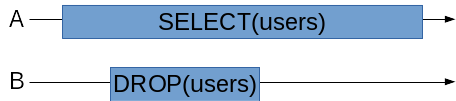
\includegraphics{concurrent_history_1}
  \caption{A possible concurrent history that OpenMemDB must be able to linearize}
  \label{concurrent_history}
\end{figure}

\par\vspace{\baselineskip}
In order to properly linearize the history in Figure \ref{concurrent_history}, we need to reorder 
the effects of the DROP operation to take place after the SELECT. Using smart pointer features 
in the language chosen for this project (C++11), we can both postpone the deletion of the 
table data while completing the DROP operation. The smart pointer guarantees the memory will 
be deleted when all references to it are released, and as the base reference (stored in the 
relation of table name to table) is removed by the DROP operation, the operation's effects 
are effectively reordered to take place after the SELECT operation.

\section{Experimental Results}
PENDING

\section{Conclusions}
PENDING

\newpage
\bibliography{WorkshopPaper}
\bibliographystyle{acm}
\newpage

\end{document}
